After the high level components were designed, the user stories helped create a more detailed view of them. At that point of
time the project focused on sprint one which meant focusing on evaluating individuals over a network.
User stories helped identify how user was going to approach the framework hence it was able to create components with known
input and return parameters. The result was a high level view of first sprint with all of it's components identified see figure ~\ref{fig:firstSprint}

\begin{figure}[htp]
\centering
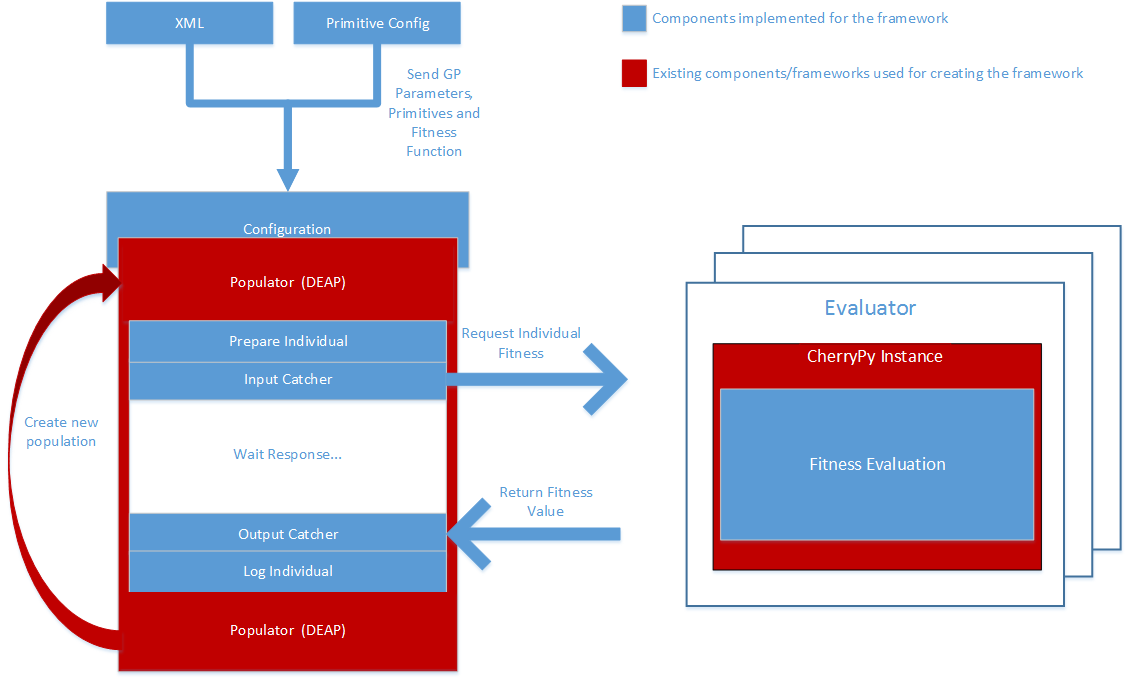
\includegraphics[scale=0.6]{Figures/FirstSprint.png}
\caption{High level view of sprint one and the identified components used}
\label{fig:firstSprint}
\end{figure}

Even though python2.7 unlike python3.3 is a semi object language for better use of software engineering practices and better ordering of the project,
objects were used to represent the different components. The diverse capabilities of python and large set of libraries helped design a complex framework with very simple architecture. Later on more 
specifics for the client design will be explained. As you can see in figure ~\ref{fig:firstSprint} Configuration, Configure Genetic Program and Genetic Program represent the three main components of the client and
CherryPy with an evaluation component represents the evaluating web service. This design helped us insert the technologies we are using at the correct
places. For example Input Catcher and Output Catcher were later on substituted by a single component that using the requests library handles the requests
and logs the traffic to the evaluator. These steps from top to down helped us clearly identified the classes that are going to be in the components.